\documentclass{exam}
\usepackage[utf8]{inputenc}
\usepackage{lmodern}
\usepackage{microtype}

% \usepackage[parfill]{parskip}
\usepackage[dvipsnames]{xcolor}
\usepackage{amsmath}
\usepackage{amsfonts}
\usepackage{amsthm}
\usepackage{siunitx}
\DeclareSIUnit\year{yr}
\DeclareSIUnit\foot{ft}
\DeclareSIUnit\litre{\liter}

\usepackage{skull}

\usepackage{pgfplots}
\usepgfplotslibrary{polar}
\pgfplotsset{compat=1.11}
\usepgfplotslibrary{statistics}
\usepackage{graphicx}
\usepackage{sidecap}
\sidecaptionvpos{figure}{c}
\usepackage{float}
\usepackage{gensymb}
\usepackage{tkz-euclide}
\usetkzobj{all}
\usepackage{commath}
\usepackage{hyperref}
\usepackage{enumitem}
\usepackage{wasysym}
\usepackage{multicol}
\usepackage{mathtools}
\usepackage{tcolorbox}
\usepackage{tabularx}
\usepackage[version=4]{mhchem}
\usepackage{changepage}
\usepackage{listings}
\lstset{basicstyle=\ttfamily\linespread{0.8}\small}

\renewcommand*{\thefootnote}{\fnsymbol{footnote}}

\newtheorem*{thm}{Theorem}
\newtheorem*{iden}{Identity}
\newtheorem*{lemma}{Lemma}
\newtheorem{obs}{Observation}
\theoremstyle{definition}
\newtheorem*{defn}{Definition}
\newtheorem*{ex}{Example}
\newtheorem{con}{Construction}
\newtheorem*{alg}{Algorithm}

\newtheoremstyle{break}
  {\topsep}{\topsep}%
  {\itshape}{}%
  {\bfseries}{}%
  {\newline}{}%
\theoremstyle{break}
\newtheorem*{bthm}{Theorem}

% russian integral
\usepackage{scalerel}
\DeclareMathOperator*{\rint}{\scalerel*{\rotatebox{17}{$\!\int\!$}}{\int}}

% \DeclareMathOperator*{\rint}{\int}

\pgfplotsset{vasymptote/.style={
    before end axis/.append code={
        \draw[densely dashed] ({rel axis cs:0,0} -| {axis cs:#1,0})
        -- ({rel axis cs:0,1} -| {axis cs:#1,0});
    }
}}

% \pointsinrightmargin
\boxedpoints
\pointname{}

\newcommand{\questioA}{\question[\texttt{\textbf{\color{Cerulean} A}}]}
\newcommand{\questioM}{\question[\texttt{\textbf{\color{PineGreen} M}}]}
\newcommand{\questioE}{\question[\texttt{\textbf{\color{WildStrawberry} E}}]}
\newcommand{\questioS}{\question[\texttt{\textbf{\color{Goldenrod} S}}]}
\newcommand{\questioO}{\question[\texttt{\textbf{\color{BurntOrange} O}}]}

\newcommand{\parA}{\part[\texttt{\textbf{\color{Cerulean} A}}]}
\newcommand{\parM}{\part[\texttt{\textbf{\color{PineGreen} M}}]}
\newcommand{\parE}{\part[\texttt{\textbf{\color{WildStrawberry} E}}]}
\newcommand{\parS}{\part[\texttt{\textbf{\color{Goldenrod} S}}]}
\newcommand{\parO}{\part[\texttt{\textbf{\color{BurntOrange} O}}]}

\newcommand{\subparA}{\subpart[\texttt{\textbf{\color{Cerulean} A}}]}
\newcommand{\subparM}{\subpart[\texttt{\textbf{\color{PineGreen} M}}]}
\newcommand{\subparE}{\subpart[\texttt{\textbf{\color{WildStrawberry} E}}]}
\newcommand{\subparS}{\subpart[\texttt{\textbf{\color{Goldenrod} S}}]}
\newcommand{\subparO}{\subpart[\texttt{\textbf{\color{BurntOrange} O}}]}

\newcommand{\mainHeader}[2]{\section*{NCEA Level 2 Mathematics\\#1. #2}}
\newcommand{\mainHeaderHw}[2]{\section*{NCEA Level 2 Mathematics (Homework)\\#1. #2}}
\newcommand{\seealso}[1]{\begin{center}\emph{See also #1.}\end{center}}
\newcommand{\drills}[1]{\begin{center}\emph{Drill problems: #1.}\end{center}}
\newcommand{\basedon}[1]{\begin{center}\emph{Notes largely based on #1.}\end{center}}

\begin{document}

\mainHeaderDiffHw{9}{Implicit Differentiation}
\subsection*{Reading}
Underpinning all our work this week was the idea that if an implicit formula in $ x $ and $ y $ is `nice enough' then there is a way to
find a `function' from $ x $ to $ y $ that we can differentiate. This rather vague notion is formalised by the rather important \emph{implicit
function theorem}, which states that if an equation $ F(x,y) = 0 $ has solution $ (x,y) = (a,b) $ then, under certain conditions\footnote{~Essentially,
that the graph of the function is not `vertical' at $ (a,b) $.}, the equation implicitly defines in some region around $ x $ a function with
a continuous derivative that takes the value $ b $ at $ x = a $ --- in other words, there is some function whose graph is the graph of $ F(x,y) = 0 $
for all of the points around the point $ (a,b) $ that we care about.

The proof of the theorem is long and we won't attempt it here; the important thing to take away is that this notion of taking a graph and then
looking at the function which it describes in a small region is well-defined, and well-defined in such a way that we can do calculus on it.

\subsection*{Questions}
\begin{questions}
  \question Find $ y' $ in each case:
    \begin{multicols}{3}
    \begin{parts}
      \part $ y^2 = x^3 + 3x^2 $\\(Tschirnhausen cubic)
            \begin{center}
              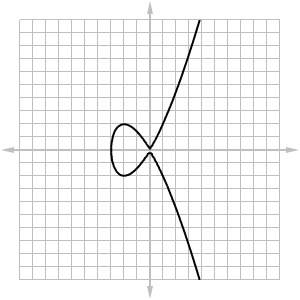
\includegraphics[width=\linewidth]{implicit10}
            \end{center}
      \part $ \sin(x + y) = 2x - 2y $
            \begin{center}
              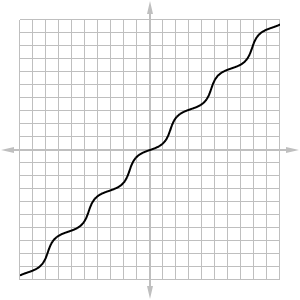
\includegraphics[width=\linewidth]{implicit11}
            \end{center}
      \part $ y^2 = 5x^4 - x^2 $\\(kampyle of Eudoxus)
            \begin{center}
              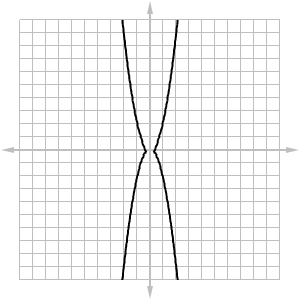
\includegraphics[width=\linewidth]{implicit12}
            \end{center}
    \end{parts}
    \end{multicols}
  \question Find the equation of the normal line to the curve $ x^2 + 2xy - y^2 + x = 2 $ at the point $ (1, 2) $.
  \question Show that the sum of the $ x $ and $ y $ intercepts of any tangent line to the curve $ \sqrt{x} + \sqrt{y} = \sqrt{c} $
            is just $ c $.
\end{questions}
\end{document}
